\SourceLeaf{116}

\clearpage\begin{center}[11.]\end{center}

\noindent\begin{minipage}[t]{.46\textwidth}
\vspace{0pt}
\[
\begin{gathered}
\beta+\varepsilon+\lambda=\boldsymbol{A}, \\
\gamma+\alpha+\lambda=\boldsymbol{B}, \\
\delta+\beta+\lambda=\boldsymbol{C}, \\
\varepsilon+\gamma+\lambda=\boldsymbol{D}, \\
\alpha+\delta+\lambda=\boldsymbol{E},
\end{gathered}
\]

\[
\begin{gathered}
\gamma+\delta+\lambda=\boldsymbol{A}', \\
\delta+\varepsilon+\lambda=\boldsymbol{B}', \\
\varepsilon+\alpha+\lambda=\boldsymbol{C}', \\
\alpha+\beta+\lambda=\boldsymbol{D}', \\
\beta+\gamma+\lambda=\boldsymbol{E}',
\end{gathered}
\]

\end{minipage}\hfill\begin{minipage}[t]{.50\textwidth}
\vspace{0pt}
\begin{center}\resizebox{5.1cm}{!}{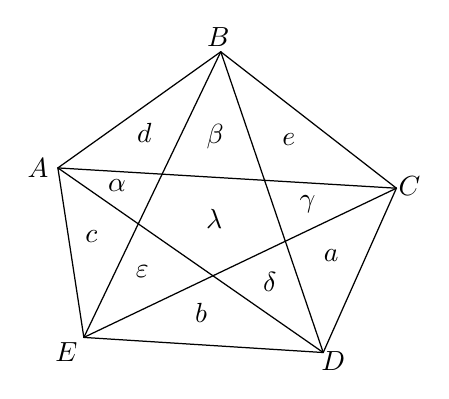
\begin{tikzpicture}[x=.006cm,y=-.006cm,line width=.45pt,line cap=round,line join=round,every node/.style={inner sep=0pt,font=\normalsize}]
\coordinate (A) at (177,347);
\coordinate (B) at (522,101);
\coordinate (C) at (894,390);
\coordinate (D) at (739,738);
\coordinate (E) at (232,706);
\draw (A) -- (B);
\draw (B) -- (C);
\draw (C) -- (D);
\draw (D) -- (E);
\draw (E) -- (A);
\draw (A) -- (C);
\draw (A) -- (D);
\draw (B) -- (E);
\draw (B) -- (D);
\draw (C) -- (E);
\node at (135,347) {$A$};
\node at (517,70) {$B$};
\node at (922,385) {$C$};
\node at (760,756) {$D$};
\node at (195,738) {$E$};
\node at (360,272) {$d$};
\node at (510,280) {$\beta$};
\node at (666,286) {$e$};
\node at (302,384) {$\alpha$};
\node at (706,424) {$\gamma$};
\node at (508,456) {$\lambda$};
\node at (248,493) {$c$};
\node at (356,566) {$\varepsilon$};
\node at (756,533) {$a$};
\node at (626,588) {$\delta$};
\node at (480,655) {$b$};
\end{tikzpicture}
}\end{center}

\[
\begin{gathered}
c+d+\alpha=\mathfrak{A}, \\
d+e+\beta=\mathfrak{B}, \\
e+a+\gamma=\mathfrak{C}, \\
a+b+\delta=\mathfrak{D}, \\
b+c+\varepsilon=\mathfrak{E},
\end{gathered}
\]
\end{minipage}


\[
a+b+c+d+e=s,
\]
\[
\alpha+\beta+\gamma+\delta+\varepsilon=\sigma,
\]
\[
\boldsymbol{A}+\boldsymbol{B}+\boldsymbol{C}+\boldsymbol{D}+\boldsymbol{E}=\boldsymbol{S}=\boldsymbol{A}'+\boldsymbol{B}'+\boldsymbol{C}'+\boldsymbol{D}'+\boldsymbol{E}',
\]
\[
\mathfrak{A}+\mathfrak{B}+\mathfrak{C}+\mathfrak{D}+\mathfrak{E}=\mathfrak{S},
\]
\[
\boldsymbol{S}=2\sigma+5\lambda=\boldsymbol{S}',
\]
\[
\mathfrak{S}=\sigma+2s, \qquad \omega=s+\sigma+\lambda.
\]

Proportionalitäten:
\[
a\boldsymbol{A}=(e+\gamma)(b+\delta),
\]
\[
b\boldsymbol{B}=(a+\delta)(c+\varepsilon),
\]
\[
c\boldsymbol{C}=(b+\varepsilon)(d+\alpha),
\]
\[
d\boldsymbol{D}=(c+\alpha)(e+\beta),
\]
\[
e\boldsymbol{E}=(d+\beta)(a+\gamma),
\]
